%% android.tex
%% by Simon Danner

% The Computer Society requires 12pt.
\documentclass[12pt,journal,compsoc]{IEEEtran}
\usepackage[ngerman]{babel}   
\usepackage[utf8]{inputenc}   % UTF8-Kodierung für Umlaute
\usepackage{hyperref}         % Hyperlinks
\usepackage{listings}
\usepackage{graphicx}
\usepackage{color}
\usepackage[usenames,dvipsnames,svgnames,table]{xcolor}

\clubpenalty = 10000           % Keine "Schusterjungen"
\widowpenalty = 10000          % Keine "Hurenkinder"

\selectlanguage{ngerman}

\newcommand{\Monat}{%
\ifcase\month
 Monat 0 \or Januar \or Februar \or März  \or April\or Mai\or Juni\or Juli\or August\or 
 September\or Oktober\or November\or Dezember
\fi}


\newcommand{\paperTitle}{
	Connecting Android powered devices to the external world	
}

\newcommand{\paperSubTitle}{
}

\newcommand{\absatz}{
	\parskip 12pt
}

\newcommand{\paperAuthor}{Simon~Danner}

\newcommand{\todo}[1]{
    \textbf{Todo:}#1
}


% korrigiere Silbentrennung % Kann man auch dazu verwendet die Silbentrennung zu deaktivieren
\hyphenation{op-tical net-works semi-conduc-tor}
% Silbentrennung für ein einzelnes Wort deaktivieren geht mit:
% \mbox{wort}

\definecolor{mybgcolor}{HTML}{DFF56C}

\lstset{
	backgroundcolor=\color{white},
	basicstyle=\footnotesize,
	breakatwhitespace=false,
	breaklines=false,
	commentstyle=\color{blue},
	stepnumber=1,
	frame=single,
	captionpos=b
}


% Bei einem zwei Spalten Layout versucht Latex auf beide Seiten die gleiche Texthöhe hinzubekommen
% Dies verursacht leider manchmal Leeräume z. B. zwischen der Überschrift und dem Text
% Mit der Option \raggedbottom kann dies unterbunden werdne
% Hat aber den Nachteil das das Dokument so einen unregelmäßigen Seitenfuß hat
% Aber immer noch besser wie die Leerräume
%\raggedbottom

\begin{document}

\title{\paperTitle \\ \paperSubTitle }
\author{\paperAuthor,~\IEEEmembership{ AI7 }}% <-this % stops a space

% The paper headers
% \markboth{Journal of \LaTeX\ Class Files,~Vol.~6, No.~1, January~2007}
% {Shell \MakeLowercase{\textit{et al.}}: Bare Advanced Demo of IEEEtran.cls for Journals}

\IEEEtitleabstractindextext{%
	\begin{abstract}
		In diesem Paper werden verschiedene Möglichkeiten der Anbindung von externen Geräten mit Android Geräten betrachtet. Dabei liegt der Fokus auf dem Android Open Accessory Protokoll. Das Protokoll sowie eine Beispielsanwendung, welche das IOIO Board verwendet werden beschrieben.
		Dabei soll gezeigt werden, wie es App-Entwicklern mit den gängigen Android Tools durch auf AOA aufbauende Hardware möglich wird mit externen Geräten zu interagieren.
	\end{abstract}

	% Note that keywords are not normally used for peerreview papers.
	\begin{IEEEkeywords}
		Android, Hardware, Arduino, IOIO, ADK, ADK 2012, AOA, Mikrocontroller   
	\end{IEEEkeywords}
}

\maketitle

\section{Einleitung}


\IEEEPARstart{A}{}ndroid ist mit einem Marktanteil von ca. 85\% das zur Zeit am weitesten verbreitete Smartphone und Tablet Betriebssystem.\cite{marketshare}
Android wird auf Smartphones, Tablets, Smartwatches, Fernsehern und anderen Geräten verwendet.
In den meisten Geräten auf denen Android verwendet wird, gibt es zahlreiche Sensoren, wie Kameras, GPS, Mikrofone und ähnliches.
Die weite Verbreitung, die Austattung sowie die Mobilität der Hardware, machen Android Geräte für eine Vielzahl von Anwendungen bei denen externe Peripherie angeschlossen werden soll, interessant.
Für Entwickler von Systemen auf Mikrocontroller Basis gibt es die Möglichkeit Daten von angeschlossenen Android Geräten zu verwenden, oder diese als Steuergerät zu nutzen.
Andererseits ermöglicht die Anbindung von externen Geräten für Entwickler welche sich mit Smartphone Anwendungen beschäftigen die Verwirklichung ganz neuer Kategorien von Applikation. 
So können zum Beispiel Anwendungen in den Bereichen Quantified Self und Hausautomation realisiert werden. 
Heute müssen Entwickler aus die für den Anwendungsfall am besten passende Möglichkeiten auswählen, um ihre externen Geräte mit Android Geräten zu verbinden.

\begin{figure}
	\centering
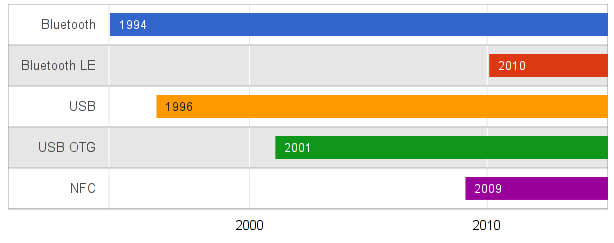
\includegraphics[width=\linewidth,angle=0]{media/chart.png}
\caption{Entwicklung von Standards}
\label{gchart}
\end{figure}




% Datum
\hfill{\the\day~\Monat, \the\year  }

\section{Allgemeines}
In diesem Paper sollen die verschiedenen Möglichkeiten der Verbindung von Android Geräten mit externen Geräten aufgezeigt, kurz beschrieben und ihr Nutzungsbereich analysiert werden.

In den letzten Jahren wurden sowohl neue Standards etabliert, sowie alte Standards optimiert um die Technologien auch in mobilen Geräten verwendbar zu machen.
So wurden Bluetooth und USB angepasst, und neue Technologien wie NFC entwickelt.\ref{gchart}
Dabei liegt der Fokus im Bereich der externen Geräte, welche mit Mikrocontroller Systemen umgesetzt sind, da mit ihnen vielfältige Hardwareprojekte auch von Amateuren entwickelt und umgesetzt werden können.

\section{Anbindungsmöglichkeiten}
Um Android Geräte mit Peripherie Geräten zu verbinden, gibt es mittlerweile mehrere Möglichkeiten.
Diese decken ein großes Spektrum an realisierbaren Anwendungen ab, wobei bei jeder Realisierung zuerst die Vorteile und Nachteile der Anbindungen analysiert werden sollte.
Nach ersten experimentellen Ansätzen von Hobbyentwicklern und einzelnen Firmen, hat auch Google den Nutzen einfacher Verbindung mit externen Geräten 
erkannt und bietet seit 2011 ein offiziell unterstütztes Protokoll, was die Entwicklung vereinfachen kann.
Dabei ist neben den verbreiteten, hardwareunabhängigen Verbindungsmöglichkeiten wie Bluetooth und NFC vor allem die Anbindung über das AOA Protokoll interessant. 

\section{Bluetooth}
Mit dem Bluetooth Standard ist es seit den 90er Jahren möglich, Geräte miteinander über Funk zu verbinden. Bluetoothschnittstellen gehören schon lange zur Standardaustattung bei Handys, Smartphones und Zusatzgeräten wie Headsets.
Die weite Verbreitung macht Bluetooth für Hardwarehersteller von Unterhaltungselektronik sehr attraktiv, da die Hardware meist einfach auf allen Betriebssystemen verwendbar ist.
Zwar müssen für spezielle Geräte Treiber entwickelt werden, jedoch ist die Unterstützung für Standardgeräte wie Headsets oder Lautsprecher schon in den meisten Betriebssystemen enthalten.

Der Standard beihaltet für die Unterstützung verschiedener Geräteklassen sogenannte Profile, welche festlegen wie diese Geräte untereinander kommunizieren.
Beispiele für oft verwendete Profile sind HID (Human Interface Devices) und OBEX (Datei Transfer). 
Durch die Standardisierung ist sichergestellt dass die Geräte untereinander kompatibel sind, und dadurch vom Endanwender ohne besondere Konfiguration verwendet werden können.
\cite{bluetooth}

Für die Anbindung von eigener Hardware können alle von Android unterstützen Profile verwendet werden. Hier kann zum Beispiel das Bluetooth Serial Port Profile (SPP) zur einfachen Übertragung von Daten genutzt werden.
Eigene Implementierungen müssen somit einen Bluetoothchip der dieses Profil unterstützt verwenden.
Zur Anbindung von selbst entwickelter Hardware ist Bluetooth aber nur bedingt geeignet, da die elektro-technische Umsetzung recht teure Chips erfordert, und ein Bluetooth Softwarestack sehr kompliziert ist. Außerdem ist der Stromverbrauch zur Übermittlung der Signale recht hoch.
Zwar ist der Stromverbrauch bei einer Übertragung von Daten über Bluetooth gering, wenn man aber die begrenzte Bandbreite berücksichtigt, hat Bluetooth gegenüber WI-Fi einen in etwa 10-fachen Stromverbrauch.\cite{wireless}
Es ist also nur für Übertragungen mit geringer Bandbreite geeignet, dort bietet es aber auf Grund der einfachen Bedienung eine benutzerfreundliche Möglichkeit der Vernetzung.

\subsection{Bluetooth Low Energy}
Um die Probleme von Bluetooth bezüglich des Stromverbrauches zu adressieren, wurde 2009 Bluetooth Low Energy, kurz Bluetooth LE, als optionaler Teil des Bluetooth Standard Version 4.0 eingeführt.  
Ziel von BLE ist es, den Stromverbrauch mittels darauf optimierter Protokolle und anderer Einschränkungen gegenüber Bluetooth zu verringern.
Die Komplexität wird unter anderem durch die Verringerung der unterstützen Profile erreicht. Klassische Bluetooth Profile wie zum Beispiel HSP (Headset), OBEX (Datei Übertragungen) und FTP (Datei Übertragungen) sind beispielsweise nicht mehr im Standard enthalten.
Dadurch werden die Treiber die Bluetoothchips verwenden einfacher und es wird möglich Bluetooth auch auf Mikrocontrollern mit beschränkten Ressourcen zu verwenden.
Energie wird durch ein neues Kommunikationsprotokoll gespart, bei der die Geräte im Standby(auf Verbindung wartend) mit weniger Energie auskommen.
Die Geräte können über eine Distanz von circa 10 Metern miteinander kommunizieren.

Mit Bluetooth 4.0 wurde auch eine neue Kommunikationsmethode, das Attribut Protokoll (ATT) eingeführt, das von Bluetooth LE verwendet und auf kleine Packetgrößen optimiert ist. 
Dadurch wird der Protokolloverhead minimiert.
Die unterstützten Profile bauen alle auf GATT auf, welches ATT benutzt um Profile bereitzustellen.

In Smartphones wurde BLE in nennenswertem Umfang zuerst von Apple mit iOS 5  Oktober 2011) unterstützt.
Dabei besitzen die Geräte sogenannte Dual-mode Bluetooth Schnittstellen, die sowohl die klassische Bluetooth als auch BLE Geräte unterstützen.
Bei Android wurde die dieses Bluetooth LE Unterstützung in der Version 4.3 (Release Juli 2013) eingeführt.

Für Hobby Entwickler, die mit Mikrocontrollern arbeiten gibt es mit Arduino kompatible Development Kits wie das nRF51, die das Board sowie Software enthalten.
Die billigeren sind für etwa \textdollar{100} erhältlich sind.
BLE lohnt sich vor allem für Hersteller von Massenprodukten die platformunabhängige Produkte herstellen wollen.
Für einfache Projekte können die Development Kits verwendet werden, allerdings ist hier mit einer hohen Komplexität bei der Implementierung der Firmware für die Mikrocontrollern zu rechnen.

\section{Near Field Communication}
Near Field Communication (NFC) ist ein Standard zu Datenübertragung über sehr kurze Strecken ( wenige Zentimeter). 
NFC findet vor allem in verschiedenen Zahlungssystemen Verwendung.
Bei diesen können Kunden mit Hilfe von Karten die NFC Chips enthalten Zahlungen tätigen.

Android unterstützt NFC seit Version 2.3. Allerdings besitzen nur wenige Smartphones die nötige NFC Hardware um NFC nutzen zu können.
Bei Android wird es auch für die Funktion Android Beam benutzt. 
Damit können Dateien von einem Android Gerät auf ein anderes übertragen werden können, ohne eine feste Verbindung einzurichten die auch ohne Konfiguration der Nutzer funktioniert.
Um von einem Android Gerät aus NFC Tags zu lesen und zu schreiben, bietet Google die NFC API an.
Durch die beschränkte Reichweite, Bandbreite und geringe Verfügbarkeit von Android Geräten, welche NFC unterstützen, empfiehlt sich NFC nur für sehr spezielle Anwendungen.

\section{Audio}
Android unterstützt Entwickler bei der Einbindung von Audio Geräten. Das Verwalten der Hardware wird von Android komplett übernommen.
Falls gewünscht, können Entwickler von Audio Applikationen über den AudioManager herausfinden, was für Geräte angeschlossen sind. So kann man zum Beispiel die Lautstärke anpassen wenn ein Bluetooth Headset verbunden wird, oder Kopfhörer entfernt werden.

Da die Verwendung von Audio Geräten fast automatisch abläuft, wird hier nicht weiter auf Audio Geräte eingegangen.

Als Kuriosität können einige Entwicklungen, bei denen die Audioausgabe zur Übermittlung an externe Geräte verwendet wird, betrachtet werden.
Diese sind im Normalfall jedoch in Anbetracht heutiger Möglichkeiten bei Neuentwicklungen nicht zu berücksichtigen.  
Ein Beispiel für ein solches Projekt ist Project HiJack \cite{hijack} , welches eine Hard- und Software Plattform zur Übermittlung von Signalen und Verarbeitung dieser auf Mikrocontrollern ermöglichte, noch bevor es von den Herstellern vorgesehene Möglichkeiten gab. 
Die Daten werden dabei analog übertragen und von dem empfangenden Gerät wieder digitalisiert.
Die Probleme hierbei sind vor allem die Komplexität, die begrenzte Bandbreite und die mangelnde Unterstützung seitens der Hersteller.

\section{USB}
Der Universal Serial Bus (USB), ist schon seit langem die am weitesten verbreitete Schnittstelle zwischen PCs und Peripheriegeräten.
Die USB Schnittstelle hat mittlerweile in vielen Bereichen wie zum Beispiel der Anbindung von Mäusen, Tastaturen und Festplatten andere speziellere Schnittstellen verdrängt.
Auch die meisten Telefone besitzen seit geraumer Zeit USB-Schnittstellen. Diese wurden anfangs vor allem zur Übertragung von Daten von und zu PCs benutzt sowie für das Laden des Akkus.
Durch die Standardisierung von Anschlüssen und Protokollen, die Möglichkeit des hinzufügens und entfernen von Geräten im laufendem Betrieb und gute Softwareunterstützung ist USB für Anwender einfach und intuitiv zu bedienen.

Technisch gesehen ist USB ein serielles Bussystem, das heißt Daten werden sequentiell zwischen den Geräten übertragen. 
Die Koordination der angeschlossenen Geräte (Slaves) wird durch einen Controller (Master) übernommen.
Slaves dürfen nur Daten über den Bus schicken, wenn sie vom Master dazu aufgefordert werden.
Im normalen Gebrauch übernimmt der PC die Rolle des Masters, die Geräte sind Slaves. Die Stromversorgung der Slaves kann dabei über das gleiche Kabel durch den Master erfolgen, wenn der Verbrauch im Rahmen des Standards liegt (5V, 500mA bei USB Version 2).

Um angeschlossene Geräte verwenden zu können, muss der Master das Gerät identifizieren können. 
Die Erkennung läuft bei hierbei über sogenannte Deskriptoren, von denen jedes USB Gerät beliebig viele bereitstellen kann. 
Der Device-Deskriptor enthält eine Hersteller-ID, sowie eine Geräte ID.
Im Device Deskriptor kann auch hinterlegt werden, ob das Gerät einer durch den Standard festgelegten Klasse zugehört. 
Klassen gibt es zum Beispiel für Massenspeichergeräte, Drucker und Human Interface Devices (Maus, Tastatur usw.).
Das Betriebssystem kann dann anhand des Deskriptors passende Treiber laden. Wenn das Gerät zu einer Standardklasse gehört, kann einfach der allgemeine Treiber verwendet werden. Dies ist zum Beispiel bei USB Mäusen der Fall.
Falls das Gerät zu keiner Standardklasse gehört, muss ein gerätespezifischer Treiber vom Betriebssystem verwendet werden.
Zur Übermittlung von Daten stellen die Geräte virtuelle Schnittstellen bereit, welche ein oder mehrere adressierbare Endpunkte beinhalten. Das Schaubild \ref{usbpic} zeigt den Aufbau eines USB Gerätes, das mit einem Host verbunden ist.

\begin{figure}[h]

	\centering
	\def\svgwidth{\columnwidth}
	\input{media/usb.pdf_tex}
	\caption{Aufbau eines USB Gerätes}
	\label{usbpics}
\end{figure}



Endpunkte sind vom USB Interface bereitgestellte Adressen. An sie können Daten unidirektional übertragen werden.
Das lesen des Device Descriptors läuft über den Endpunkt mit der Adresse 0, danach werden die anderen Gerätespezifischen Endpunkte ausgelesen und verwendet.

Die Kommunikation mit den Endpunkten kann über verschiedene Modi ablaufen, um verschiedene Anforderungen zu erfüllen.
Dabei unterscheiden sie sich zum Beispiel bei der Bestätigung von Nachrichten oder der Priorisierung.  

\subsection{USB On-The-Go}
USB On-The-Go (OTG) ist eine Spezifikation, die USB Geräten erlaubt dynamisch zwischen verschiedenen Betriebsmodi zu wechseln. 
Im USB Standard ist festgelegt, dass jedes Gerät entweder die Rolle des Host oder des Slave einnimmt, und diese nicht geändert werden kann. 
OTG weicht diese Regeln auf, um größere Dynamik und damit neue Anwendungen zu erlauben.
OTG Geräte können auch ohne Host-Controller mit USB Geräten kommunizieren, indem das OTG Geräte zum Host wird.
Dabei muss nur ein Teil der normalen Host Funktionalität bereitgestellt werden.

Mit einigen wenigen Androidgeräten kann OTG verwendet werden.
Softwareseitig unterstützt Android seid Version 3.1 OTG,
allerdings muss die verbaute USB Hardware dafür OTG unterstützen.
Vor allem Tablets unterstützen oft OTG, damit Anwender zum Beispiel Tastaturen, Drucker oder USB Sticks verwenden können.
Als angeschlossenes Gerät unterstützt Android die durch den Linux Kernel unterstützten USB Geräte.
Eigene Hardware die mit der OTG Unterstützung kontrolliert werden könnte zu entwickeln, wäre denkbar aber durch die Komplexität von USB mit hohem Aufwand verbunden.
Es müsste ein Gerät entwickelt werden, welches eines der Standard USB Profile implementiert, um vom Gerät verwendet werden zu können, jedoch die spezifizierten Kommandos nutzt um Funktionen umzusetzen.
Daher ist die OTG nur für Hardware interessant, welche in die Kategorien des im USB Standard festgelegten Geräteklassen fällt, wie z.B eigene Tastaturen oder andere Eingabegeräte. 

\subsection{AOAP (Android Open Accessory Protokoll)}
Android Open Accessory ist der Name eines von Google entwickelten Protokolls, das 
dezidiert für die Anbindung von externen Geräten an Android Geräte entwickelt wurde.
Aufgrund der offiziellen Unterstützung und des Funktionsumfanges wird AOA hier detailliert vorgestellt.
Google stellt zum Einstieg das Accessory Development Kit (ADK) zu Verfügung mit der Entwickler relativ einfach Anwendungen die Software und Hardware kombinieren umsetzen können.
Als Accessories bezeichnet Google elektronische Zusatzgeräte, welche in der Verbindung mit dem Androidgerät neue Funktionen für den Nutzer bereitstellen.
Das ADK besteht aus einer Hardware Referenz Plattform, sowie Quellcode für diese, damit 
Entwickler einfach Hardware und Software anpassen und erweitern können.
\cite{developaoa}
\subsubsection{Ziel}
Das Ziel von Google ist es mithilfe des AOA einen einheitlichen Standard zur Verbindung von externen, selbst entwickelten oder auch industriell hergestellten Geräten mit Android Geräten zu etablieren.

Die Bereitstellung des Protokolls und die Unterstützung in allen aktuellen Androidversionen soll dazu führen, dass Endanwender ohne Vorwissen über Gerätkombinationen und Details, externe Hardware verwenden können.
Google veröffentlichte bisher (Stand November 2014) zwei Versionen des ADK, ADK 2011 und ADK 2012. 

\subsubsection{Geschichte}
Schon vor der Vorstellung des ADK gab es diverse Projekte, die das Ziel hatten Android mit Hardware auf Mikrocontroller Basis zu verbinden.
Der Standardweg dies zu bewerkstelligen war die Nutzung des Android Debug Bridge (ADB) Protokolls.
Die Unterstützung von ADB kann auf vielen Geräten vom Endanwender aktiviert werden. Dadurch kann eine Kompatibilität mit vielen Geräten erreicht werden, wenn die Kommunikation über dieses Protokoll abläuft. 
Über das Protokoll können beliebe Datenpakete geschickt werden. Zur Verwendung von Mikrocontrollern muss also eine Firmware implementiert werden, die das ADB Protokoll unterstützt und über dieses Kommandos zwischen der Android Applikation und sich selbst austauschen kann.

Gegenüber der Kommunikation über das ADB Protokoll, bietet AOA einige Vorteile. In Tabelle  \ref{table:vergl} sind einige Kenngrößen gegenüber gestellt. Der größte Vorteil der Benutzung von AOA gegenüber ADB, besteht darin, dass AOA nicht explizit vom Benutzer eingeschaltet werden muss und offiziell unterstützt wird.


\begin{table}
	\centering
	\caption{Vergleich ADB / AOA Quelle: \cite{comp}}
	\label{table:vergl}
	\begin{tabular}{c | c | c}
		& ADB & AOA \\ \hline
		Latenz & 4ms & 1ms \\ \hline
		Durchsatz & 300 KB/s & 600 KB/s \\ \hline
		Verfügbarkeit & alle Versionen & \textgreater 2.3.4 \\ \hline
	\end{tabular}
\end{table}


\subsubsection{ADK 2011}
Beim ADK 2011 wurde von Google eine
Referenz Plattform auf Basis eines Arduino Mega2560 Mikrocontroller System veröffentlicht. Das Board besitzt ein USB Host Modul was zusammen mit einer Arduino Bibliothek zur Kommunikation über das AOA Protokoll verwendet werden kann.
Durch die Benutzung des Arduino Controllers ermöglicht es Google, Hobby Entwicklern einen einfachen Einstieg in die Entwicklung von Accessoires, da diese Mikrocontroller sehr verbreitet sind.
Für Arduinos gibt es viel Software- und Hardwaremodule die einfach für eigene Projekte wiederverwendet werden können.
Die Programmierung ist mit der Arduino IDE möglich, welche einen C-Dialekt verwendet der auch für Anfänger einfach verständlich ist.
Die Android seitige Funktionalität von AOA wurde in Android 2.3.4 (Release April 2011) und spätere Versionen integriert. 
Um mit dem ADK eigene Accessoires entwickeln zu können, muss das Board zunächst mit der von Google bereitgestellten Firmware, welche AOA implementiert geflasht werden.
Auf dem Microcontroller muss für die Verwendung von AOA zunächst einige Setup Routinen aus der von Google bereitgestellten Bibliothek aufgerufen werden.

\begin{lstlisting}[language=C]
ADK L;
void setup() {
L.adkInit();
L.usbSetAccessoryStringVendor(...);
L.usbSetAccessoryStringName(...);
L.usbSetAccessoryStringLongname(...);
L.usbSetAccessoryStringVersion(...);
L.usbSetAccessoryStringUrl(...);
L.usbSetAccessoryStringSerial(...);
L.usbStart();
}
\end{lstlisting}

Danach kann mit der Arduino IDE die Funktionalität implementiert werden.

\begin{lstlisting}[language=C]
void loop() {

if (L.accessoryConnected()) {

int recvLen = L.accessoryReceive(msg, sizeof(msg));
if (recvLen > 0) {
	... // verarbeite Nachricht 
}
L.accessorySend(outmsg, outmsgLen);
}
L.adkEventProcess(); // Disconnect und 
// Event Processing
}
\end{lstlisting}

Die loop Methode wird in einer Schleife aufgerufen. Falls Nachrichten vom Android Gerät empfangen wurden können diese verarbeitet werden.

\begin{lstlisting}[language=Java]
ParcelFileDescriptor mFD = 
   mUSBManager.openAccessory(acc);
if (mFD != null) {
FileDescripter fd = mFD.getFileDescriptor();
// Lese Nachrichten vom Accessory 
mIS = new FileInputStream(fd);  
// Schreibe Nachrichten an Accessory 
mOS = new FileOutputStream(fd); 
}
\end{lstlisting}
Nach öffnen des Geräts, können aus der Android Anwendung die Nachrichten in FileStreams geschrieben werden.

Wenn das ADK so verwendet wird, muss der Entwickler festlegen in welcher Form Nachrichten übermittelt werden. 
Es könnten zum Beispiel Low-level Nachrichten verwendet werden wie "Pin 1 an" oder Highlevel Nachrichten, welche auf dem Arduino eine Reihe von Ereignissen auslösen.
Diese Flexibilität ermöglicht es das ADK in vielen Anwendungsbereichen zu nutzen.

\subsubsection{ADK 2012}
In der zweiten Version des ADK wurde die Hardware Plattform gewechselt. Nun dient ein Arduino kompatibles Board mit einem ARM Cortex M3, Sensoren für Licht, Farbe, Temperatur, Feuchtigkeit, Druck und Beschleunigung, einem Micro SD Card Slot und Bluetooth als Referenzhardware.
Die neuen Sensoren und Verbindungsmöglichkeiten machen dieses Board noch attraktiver für Entwickler, welche die Anbindung weiterer eigener Sensoren vermeiden wollen.

Mit dem ADK 2012 wurde auch das AOA Version 2 Protokoll veröffentlicht.
Es fügt die Möglichkeit von Audio Übertragungen sowie HID (Human Interface Devices) über das AOA Protokoll hinzu, wodurch Anwendungen in diesem Gebiet vereinfacht werden.
Bei dieser Art der Nutzung kommuniziert das Geräte mit dem Android Betriebssystem und nicht mit einer einzelnen Anwendung.

\lstinputlisting[language=Java]{code/bluetooth.java}
In der Android App kann über die Android Bluetooth Schnittstelle eine Verbindung aufgebaut werden.
\lstinputlisting[language=Java]{code/bluetooth2.java}
Dann kann über Streams mit dem Gerät kommuniziert werden.

\subsection{Das AOA Protokoll}
Um mit einem Android Gerät kommunizieren zu können, müssen mehrere Schritte vom externen Gerät durchgeführt werden.
Das externe Gerät agiert dabei als USB Host und versorgt das Android Gerät mit Strom.
Beim Anschließen des Gerätes an das Androidgerät wird zunächst überprüft ob das angeschlossene Gerät den Accessory Modus unterstützt.
Falls dies zutrifft, wird das Gerät auf diesen Modus umgestellt und danach die Kommunikationskanäle aufgebaut.
Erkannt wird der Accessory Modus, wenn das USB-Interface die Vendor ID 0x18D1 und die Produkt ID von 0x2D00 (für AOA) oder 0x2D01 (AOA + ADB unterstützt) besitzt.
In Version zwei kamen weitere IDs hinzu, mit denen Geräte welche auch Audio über AOA unterstützen.

Dafür werden USB Deskriptoren genutzt, um geeignete USB Endpunkte zu finden. AOA benutzt Bulk-Endpunkte. Diese werden bei USB im allgemeinen zum Transport von längeren Block-artigen Datenblöcken benutzt.

Bulk Transfers verwenden CRC zur Fehlererkennung und Korrektur. Es ist garantiert das übertragene Daten korrekt ankommen, es gibt allerdings keine Bandbreite oder Latenz Vorschriften für die implementierende Hardware.
\cite{usbbulk}
Nachdem die korrekten Endpunkte gefunden wurde, können sie von dem Accessoir zum senden von Daten verwendet werden.
Bei der Änderung des Androidgerätes in den AOA Modus, wird eine Liste von Applikationen welche die AOA API unterstützen dem Benutzer angezeigt. 
Die Liste enthält alle Applikationen, welche die für den Gebrauch von AOA nötigen Berechtigungen besitzen.
Der Benutzer kann dann die zum aktuellen Accessoir passende Applikation auswählen und das angeschlossene Gerät verwenden.

\section{Beispiel AOA Anwendung}
Da Android Open Accessory die von Google offiziell unterstützte API für die Anbindung externer Geräte ist, wird hier auf den Aufbau solcher Applikationen detaillierter eingegangen. Außerdem wird an einer Beispielsapplikation der Aufbau von Systemen, welche intern auf AOA aufbauen erläutert.
\subsection{AOA Hardware}
Um mit AOA eine Anwendung mit Hardwarekomponente entwickeln zu können, braucht man ein kompatibles Hardwareboard.
Zurzeit können hierfür die von Google als Referenz Plattform bereitgestellten Arduinos, sowie einzelne andere Boards von Drittherstellern, wie zum Beispiel das IOIO Board \cite{ioio}, oder das AOAA Kit von Embedded Artists\cite{aoaa} verwendet werden.

Falls man andere, spezielle Hardware anbinden möchte kann man auch anhand der Protokoll Spezifikation \cite{aoaprotocol2} eigene Systeme anbinden. 
Das Protokoll ist zwar recht einfach gestaltet, aber die Implementierung würde einen deutlich größeren Aufwand für viele Projekte bedeuten. 

Für die Beispielsanwendung wird das IOIO Board, welches mit Firmware welche AOA unterstützt benutzt werden kann verwendet.

\subsection{IOIO Hardware}
Die erste Version des IOIO Boards wurde im September 2011 vorgestellt. Das Board wurde von Ytai Ben-Tsvi, einem Google Angestellten, für eigene Projekte im Rahmen der Google 20\% Zeit entwickelt und als Kooperation mit dem Elektronikunternehmen SparkFun produziert und verkauft.
Es war der erste Board, welches ohne Modifikationen an Android Geräten von diesen verwendet werden konnte, um damit externe Peripherie zu steuern.
Dies wurde über die Verwendung der Android Debug Bridge erreicht, welche als Übertragungsprotokoll verwendet wird.

Als Mikrocontroller kommt ein PIC24F zum Einsatz, welcher auf Grund seiner vielen Anschlüsse und geringer Kosten gewählt wurde.
Das Board besitzt 48 Pins, welche als Digitale Inputs und Outputs angesteuert werden können. 16 dieser Pins können auch als analoge Inputs verwendet werden.
Zusätzlich können 9 PWM (Pulsweitenmodulation) Ausgänge verwendet werden.
Für die Kommunikation mit anderen Elektronischen Geräten stehen 4 UART Kanäle, 3 SPI Kanäle und 3 TWI Kanäle, welche mit I\textsuperscript{2}C kompatibel sind zur Verfügung.
Der Strom wird über ein externes 5 Volt Netzteil bereitgestellt, welches bis zu 1.5 Ampere liefern muss.

Die externe Stromversorgung ist praktisch, da sowohl das Androidgerät geladen werden kann, als auch Motoren oder ähnliches durch das Netzteil mitversorgt werden können.
Ziel der Neuentwicklung war vor allem eine kostengünstige Möglichkeit zum Einstieg in die Hardware Entwicklung mit Android verfügbar zu machen.
Mit einem Preis von \textdollar{50} ist das Referenzboard für erste Versuche mit Mikrocontrollern, individuelle Hardwarebastlereien und Prototypen geeignet.
Das Board besitzt einen USB Anschluss, welcher im Host Modus betrieben werden kann, was Voraussetzung für den Betrieb von ADB und AOA ist.

\subsubsection{IOIO-OTG}
Im Sommer 2012 wurde die zweite Version des IOIO Boards veröffentlicht.
Die größte Änderung ist die Möglichkeit das IOIO Board als USB OTG Device zu betreiben.
Dies ermöglicht die Verbindung mit PCs, mit denen das Gerät direkt programmiert werden kann.
Der Entwicklungsprozess wird dadurch vereinfacht, da keine Android Applikation mehr auf dem Gerät installiert werden muss um Programme zu testen.
Die Java Bibliothek wurde so angepasst, dass sie nicht nur unter Android sondern auch mit der Standard JVM verwendbar ist. 
Dadurch können auch Anwendungen, welche den Mikrocontroller vom PC aus verwenden erstellt werden.
Außerdem konnten die Produktionskosten weiter gesenkt werden, die neue Version ist nun bei den Partnerunternehmen des Projektes für ca. \textdollar{30} erhältlich.

\subsubsection{IOIO Anbindung}
Die IOIO Bibliotheken stellen mehrere Verbindungsmöglichkeiten bereit. Mit ihnen kann sowohl von einem Android Gerät als auch einem PC dem IOIO Board Befehle übermittelt werden.
Durch die klare Trennung von Protokoll und Übertragungsweg ist es möglich, das ,,Backend"" welches Hardware nahe Befehle enthält, ohne Modifikationen in Android und Desktop Anwendungen zu nutzen.
Das IOIO Protokoll setzt zur Übertragung entweder auf Bluetooth oder USB \ref{protocolls}.

In im sind Kommandos wie \glqq Schalte Pin 1 ein\grqq, oder \glqq Lese Pin 3 analog\grqq spezifiziert \cite{ioioprotocoll}, die durch entsprechende Methoden direkt in der zugehörigen IOIO Android Bibliothek aufgerufen werden können.
Die Firmware auf dem IOIO tut nichts, außer die Kommunikation zum Android Gerät zu unterhalten, und die low-level Kommandos die es erhält umzusetzen.
Wenn erwünscht kann auch die Firmware modifiziert werden, sie steht unter einer Open Source Lizenz zur Verfügung, allerdings benötigt der Entwickler dann C Kenntnisse.
Dadurch ist es, gegenüber dem ADK, dem Entwickler nicht möglich High-level Befehle vom Android Gerät an das IOIO Board zu übermitteln. 
Dies schränkt in manchen Fällen den Entwickler ein, da die gesamte Logik, bezüglich anzusteuernder Elektronik des Boards, auf dem Android Gerät laufen muss.
Dies kann unter anderem die Umsetzung von zeitkritischen Anwendungen, bei der zunächst ein Wert vom IOIO ausgelesen werden muss und dann darauf reagiert werden soll, durch den Kommunikations- und somit Zeitoverhead verkomplizieren.

\begin{figure}[h]

	\centering
	\def\svgwidth{\columnwidth}
	\input{media/protocols.pdf_tex}
	\caption{IOIO Protokollschichten}
	\label{protocolls}
\end{figure}



\subsection{Vorhaben}
Nachfolgend soll anhand eines einfaches Projektes die Konzepte und Möglichkeiten, sowie Probleme des IOIO Board erläutert werden. 
Das Ziel ist es eine Android App zu entwickeln, welche es ermöglicht einen Atari 2600 zu steuern.


\subsubsection{Atari 2600}
Das Atari Video Computer System (Atari VCS), kurz Atari 2600 ist ein ab 1977 vertriebene Spielkonsole. 
Es war eine der ersten Spielkonsolen, und ist bis heute mit etwa 30 Millionen verkauften Exemplaren die am meisten verkaufte.
Die verbaute Hardware ist für heutige Verhältnisse sehr beschränkt. 
So beinhaltet die Konsole 128 Byte RAM und einen Prozessor 1,19 MHz Taktfrequenz.
Mit Hilfe von einsteckbaren Modulen können Spiele geladen werden, von denen bis 1987 etwa Titel 1200 lizenziert wurden.
Angeschlossen wird das System an einen Fernseher, auf dem bis zu 128 verschiedene Farben dargestellt werden.
Es sind zwei Anschlüsse für Controller vorhanden. Von Atari wurden sowohl Standard Joysticks als auch speziellere Eingabegeräte wie Paddles verkauft.

Die Joysticks werden über 9-polige D-Sub Stecker angeschlossen.
Dabei werden bei einem Joystick 5 der Pins für die verschiedenen Richtungen und den Feuerknopf verwendet.
Die Steuerung funktioniert wie bei einfachen Schaltern von denen, durch den Aufbau des Joysticks, maximal drei gleichzeitig gedrückt werden können. ( Zwei Richtungen und der Feuerknopf)
Die Spannung am jeweiligen Pin wird beim drücken des Joysticks in eine Richtung von 5 Volt auf 0 Volt durch die Verbindung mit Ground heruntergesetzt, was vom Atari als Input erkannt wird.
Das Ziel ist es eine Android Anwendung zu schreiben, mit der von einem Smartphone die Spannung an den Input-pins manipuliert werden kann.

\subsection{Umsetzung}
Das IOIO Board wird teilweise ohne funktionsfähige Firmware ausgeliefert. Falls dies der Fall ist, muss man die Standard Firmware, welche AOA implementiert, von der Projekt Seite beziehen und selbst die Software auf die Hardware flashen.
Die Firmware übernimmt hierbei die Implementierung des AOA Protokolls, so dass der Entwickler sich auf die zu Implementierte Funktionalität konzentrieren kann.

Um ein solches Hardwareprojekt einfach und schnell umsetzen zu können, sollte man die Komplexität am Anfang beschränken, damit die Fehlersuche vereinfacht wird.
Außerdem können mit dem IOIO Framework Applikationen sowohl auf dem PC mit der Standard Java VM als auch auf Android entwickelt werden.
Am PC wird die Kommunikation mit dem IOIO über USB mit Hilfe der purejavacomm Bibliothek realisiert.
Das arbeiten auf dem PC macht es einfacher die Anwendung zu testen, da das installieren auf dem Gerät wegfällt.
Als einfachen Einstieg, und um die Funktionalität des IOIO Board zu überprüfen, bietet es sich an, zuerst eine einzelne LED zu installieren, welche von der Anwendung angesteuert werden kann.
\begin{figure}[h]
	\def\svgwidth{\columnwidth}
	\input{media/circuit.pdf_tex}
	\caption{Schaltplan für IOIO Atari Controller}
	\label{fig:circuit}
\end{figure}

Um die Pins von 5 Volt auf 0 Volt zu erreichen, werden fünf der IOIO Digitalausgänge mit den Eingängen eines Transistorarray vom Typ ULN2003A verbunden, siehe \ref{fig:circuit}.
Dies ermöglicht es, die einzelnen Pins durch den IOIO an- und abzuschalten und somit den Joystick zu emulieren.

Um den IOIO mit Android zu steuern, gibt es Bibliotheken welche in das Androidprojekt eingebunden werden kann.
Leider werden vom Projekt selbst keine .jar Dateien bereitgestellt, diese müssen entweder selbst erstellt oder anders bezogen werden. Durch die Abhängigkeiten zwischen den Bibliotheken, ist die Erstellung der Bibliotheken etwas kompliziert.

Vom Projekt werden vier Bibliotheken bereitgestellt:

\begin{itemize}
	\item IOIOLib - Basisklassen 
	\item IOIOLibAndroidDevice - USB Management für Android
	\item IOIOLibAccessory - Verbindungen über AOA
	\item IOIOLibBT - Verbindungen über Bluetooth
\end{itemize}

Die IOIOLib Bibliothek bietet Basisklassen, welche zum einen die Hardware abstrahieren, sowie Klassen für die Entwicklung von Android und PC Anwendungen.
In der IOIOLibAndroidDevice ist das Öffnen von USB Geräten unter Android Geräten implementiert.
Die IOIOLibAccessory implementiert das IOIO Protokoll über das Android AOA Protokoll, die IOOILibBT über Bluetooth.

Die IOIOLib API ist recht einfach gehalten.
So können die verschiedenen Hardwareports des IOIO über verschiedene Input und Output Klassen adressiert werden.
Um beispielsweise einen Port im Digitalmodus zu öffnen, von dem gelesen werden kann, genügt folgender Einzeiler:

\begin{lstlisting}[language=Java]
DigitalOutput led = ioio.openDigitalInput(2); 
\end{lstlisting}

Danach kann mit
\begin{lstlisting}[language=Java]
led.write(true); 
\end{lstlisting}
der Pin auf ein logisches true gesetzt werden.
Die meisten Pins können in mehreren Modi betrieben werden, was durch Schließen mit pin.close() und wieder öffnen in einem anderen Modus softwareseitig umgesetzt werden kann. 

\begin{figure}
	\centering
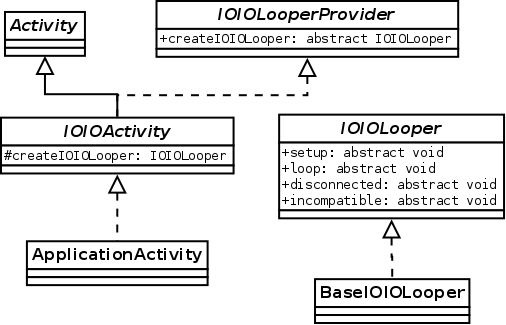
\includegraphics[width=\linewidth,angle=0]{media/classdiagram/Diagram1.png}
\caption{Klassendiagramm}
\label{fig:classdia}
\end{figure}



Um einfach Android Apps entwickeln zu können, sollte eine Klasse implementiert werden, die von IOIOActivity erbt\ref{fig:classdia}.
Diese bringt die IOIO Funktionalität in die Android Activity ein, und stellt Methoden bereit, welche von der eigenen Activity überschrieben werden.
Die wichtigste Methode ist 
\begin{lstlisting}[language=Java]
protected IOIOLooper createIOIOLooper(){};
\end{lstlisting}

welche überschrieben werden muss, um eine eigene Implementierung eines IOIOLooper zurückzugeben.

Die eigentliche Hardwarenahe Funktionalität wird in einer Klasse gekapselt, welche IOIOLooper implementiert. 
Das Interface besteht aus folgenden Methoden:

\begin{lstlisting}[language=Java,caption={Definitionen in IOIOLooper.java}]
public interface IOIOLooper{
	public abstract void setup(IOIO ioio);
	public abstract void loop();
	public abstract void disconnected();
	public abstract void incompatible();
}
\end{lstlisting}


Der Code in der Looper Klasse wird durch das IOIO Framework in einem separatem Thread abgearbeitet.
Die ,,setup'' Methode wird nach dem Aufbau einer Verbindung einmalig aufgerufen. Darin können unter anderem Pins geöffnet werden, welche dauerhaft verwendet werden.
Im Fall dass ein inkompatibles Gerät verbunden wird, also mit alter Firmware, wird die ,,incompatible'' Methode aufgerufen.
Bei einer Trennung der Verbindung wird die ,,disconnected'' Methode aufgerufen. 
Die zentrale Methode, in der fast alle Funktionalität implementiert wird, ist die ,,loop'' Methode.
Diese wird in einer Schleife immer wieder aufgerufen.
In vielen Applikationen empfiehlt es sich deswegen in der von IOIOActivity Klasse erbenden Klasse den Controller, zum Beispiel die GUI zu implementieren und eine Art Zustand zu speichern, welcher dann in der loop Methode auf den IOIO übertragen wird. 

Der Code des Beispielsprojekts ist auf GitHub verfügbar, nachfolgend sollen die Grundlagen erläutert werden. \cite{danners_github}

In der von IOIOActivity erbenden Controller Klasse, wird die Richtung aus einem Joystick GUI Element ausgelesen. Die Richtungen werden dann in booleschen Variablen abgelegt.
Diese werden von einer inneren Klasse, welche IOIOLooper implementiert ausgelesen und an den IOIO übertragen.

\begin{figure}
	\centering
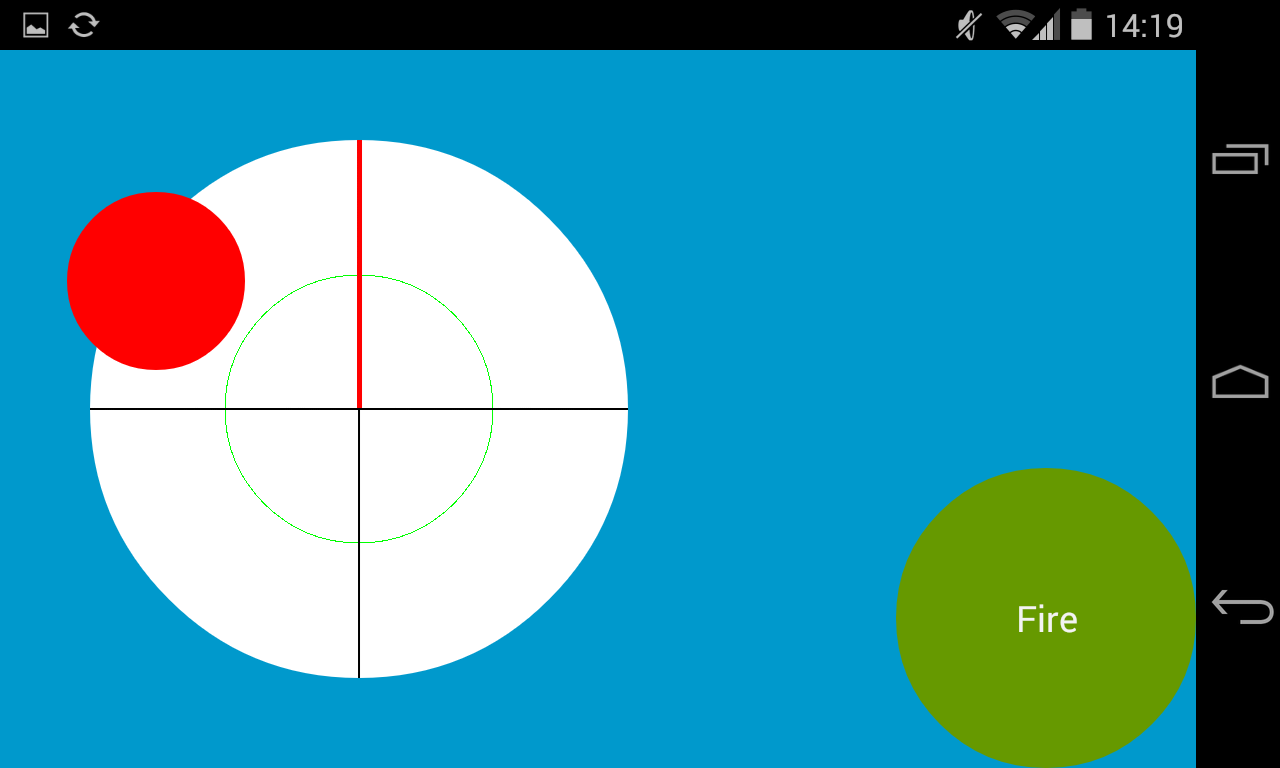
\includegraphics[width=\linewidth,angle=0]{media/screenshot.png}
\caption{Screenshot Atari Controller App}
\label{fig:atari_c}
\end{figure}

Im Atari Beispiel implementiert die Controller Klasse IOIOActivity, und stellt in createIOIOLooper eine Instanz von AtariLooper bereit. 
Es wird ein Joystick dargestellt (siehe \ref{fig:atari_c}, und ausgelesen in welcher Richtung der virtuelle Joystick ausgelenkt wird. 
Der AtariLooper öffnet bei der Verbindung eines IOIO die fünf benötigten Pins, damit die Richtungen an den Atari übertragen werden können.
Die Richtungen werden in booleschen Variablen abgelegt, welche dann durch den separaten Thread im erzeugtem AtariLooper ausgelesen und die jeweiligen Pins am IOIO aktiviert werden. 

\subsection{Erkenntnisse}

Die Umsetzung dieses Hardware Projekts ist auch für Anfänger, die wenig Erfahrung mit Mikrocontrollern möglich.
Das IOIO Board ist einfach zu benutzten und bietet viele Möglichkeiten Schaltkreise anzubinden und zu kontrollieren.
Durch die Verfügbarkeit der IOIO Bibliotheken auf dem PC ist das Testen der Hardware einfach umsetzbar.

Der größte Vorteil gegenüber anderen Mikrocontrollern ist dass die Firmware bereits das AOA Protokoll implementiert. Dadurch wird es auch Anfängern möglich Hardware mit Androidgeräten anzusteuern. 

Bei der Implementierung des Beispielprojekts wurden jedoch auch einige Schwächen ersichtlich.
So ist die Dokumentation unorganisiert, teilweise veraltet und nur in einem Wiki gesammelt.
Dass die Bibliotheken nur als Eclipse Projekte zum Download bereitgestellt werden, macht den Einstieg schwerer als nötig. Diese selbst zu erstellen ist schwierig, da die einzelnen Projekte untereinander Abhängigkeiten besitzen.

Ab Android 4.2 ist die Kommunikation über das ADB Protokolls defekt, da mit dieser Version secure ADB eingeführt wurde, was momentan nicht von der IOIO Firmware implementiert ist. ADB wird jedoch als Standard Transport Protokoll benutzt.
Deswegen ist beim Testen mit einem Android Gerät darauf zu achten, das USB-Debugging zu deaktivieren, sonst kommt es zu schwer nachvollziehbaren Fehlern.
Diese Notwendigkeit macht die Entwicklung mit echten Geräten jedoch sehr umständlich, da das USB Debugging ständig an ( für das installieren der App) und ausgeschaltet (für das Testen mit dem IOIO) werden muss.
Der Hauptentwickler ist sich des Problemes bewusst \cite{adbbroken}, verweist jedoch auf die Möglichkeit die Anwendung mit AOA zu benutzen oder mit einer Desktop Applikation zu testen. 

\section{Ausblick}
Da es für neue Projekte oft wichtig sein kann, dass sie auch in der Zukunft funktionieren, muss vor der Systemkonzeption auch auf die Entwicklung der verwendeten Technologie eingegangen werden.
Nachfolgend wird kurz auf bereits absehbare, voraussichtliche Entwicklungen der verschiedenen Anbindungsmöglichkeiten eingegangen. 
\subsection{AOA}
Seit dem Release der aktuellen Version 2012 gab es keine Ankündigungen für Neuerungen.
\subsection{Bluetooth}
Android 5 unterstützt nun auch Bluetooth Version 4.1. In der neuen Version werden Probleme mit Störungen des 4G Empfanges durch Bluetooth behoben, da Bluetooth 4.0 und LTE die gleichen Frequenzen verwenden.
Dies führt zu einer höheren Zuverlässigkeit der Verbindungen mit externen Geräten.
Außerdem ermöglicht Bluetooth 4.1 dass Geräte gleichzeitig als Hub und Slave agieren.
Dies ermöglicht es zum Beispiel gleichzeitig von einem Accessory Daten einzusammeln und mit einem Bluetoothheadset verbunden zu sein.
Das macht die Anbindung von externen Geräten mit Bluetooth um einiges attraktiver, allerdings setzt die Hardware in aktuellen Geräte noch nicht die neue Spezifikation um.
\subsection{NFC}
Mit Android 5 kann nun der Sperrbildschirm entsperrt werden, wenn ein bestimmter, vom Benutzer konfigurierter NFC Tag in Reichweite ist. Zur Anbindung externer Hardware ist dies aber nur bedingt interessant.


\subsection{USB}
In der Android Version L, welche im Herbst 2014 veröffentlicht wurde, unterstützt USB audio-out. Mit USB Audio-out lässt sich, anders als bei den Klinkenbuchsen, der Smartphone interne Digital-Analog-Umsetzer umgehen. Das ermöglicht es Soundtechnikern bessere, externe DAUs zu verwenden.
Dadurch kann Musik produziert, Mischpulte gesteuert und USB Kopfhörer verwendet werden.
Damit zieht Google mit Apple gleich, welche die Technik schon seit 
Das ermöglicht das Verwenden von USB Geräten  
Um USB audio-out verwenden zu können, wird ein OTG kompatibles Gerät benötigt.

\section{Fazit}
Für die Anbindung von externen Geräten ist für Hobby Entwickler Hardware wie das IOIO Board zu empfehlen.
Da die Kommunikation zum Mikrocontroller durch die bereitgestellten Bibliotheken abläuft, kann sich ganz auf die eigentliche Anwendung konzentriert werden, ohne eigene hardwarenahe Protokolle selbst zu implementieren.

Das Android Open Accessory Protokoll stellt für Hersteller von Mikrocontrollern eine Chance dar, es ihren Anwendern zu ermöglichen Android für eigene Anwendungen zu nutzen.
Sieht man von Schwächen bei der Dokumentation und den Grundeinstellungen ab, ist das IOIO Board mit den dazugehörenden Bibliotheken zu empfehlen, wenn ein Projekt schnell und unkompliziert umgesetzt werden soll.
Falls ein Projekt massengefertigt werden soll, würde man aber wohl zur Kostensenkung auf einen individuell angepasstes Board, welches AOA implementiert ausweichen.




\bibliographystyle{IEEEtran}
\bibliography{android_quotes}

% for the book
\nocite{*}
\end{document}

